%!TEX root = ../../main.tex
\section{Metoder}

I dette projekt er der blevet brugt følgende arbejdsmetoder:
\begin{itemize}
	\item V-Modellen
	\item SCRUM
	
\end{itemize}

\subsection{V-Modellen}

V-Modellen, som er en udviklingsmodel, er blevet brugt til at lave løbende test i dette projekt. Da der laves test sideløbende sikres der, at systemet virker efter hensigten. På figur \ref{VModel} kan V-Modellen ses. V-Modellen er valgt at arbejde ud fra, da det at teste systemet er noget der er lært løbende på semestret og med V-Modellen sikres der at det lærte stof kan anvendes sideløbende med udviklingen af projektet. 

\begin{figure}[H]
	\centering
	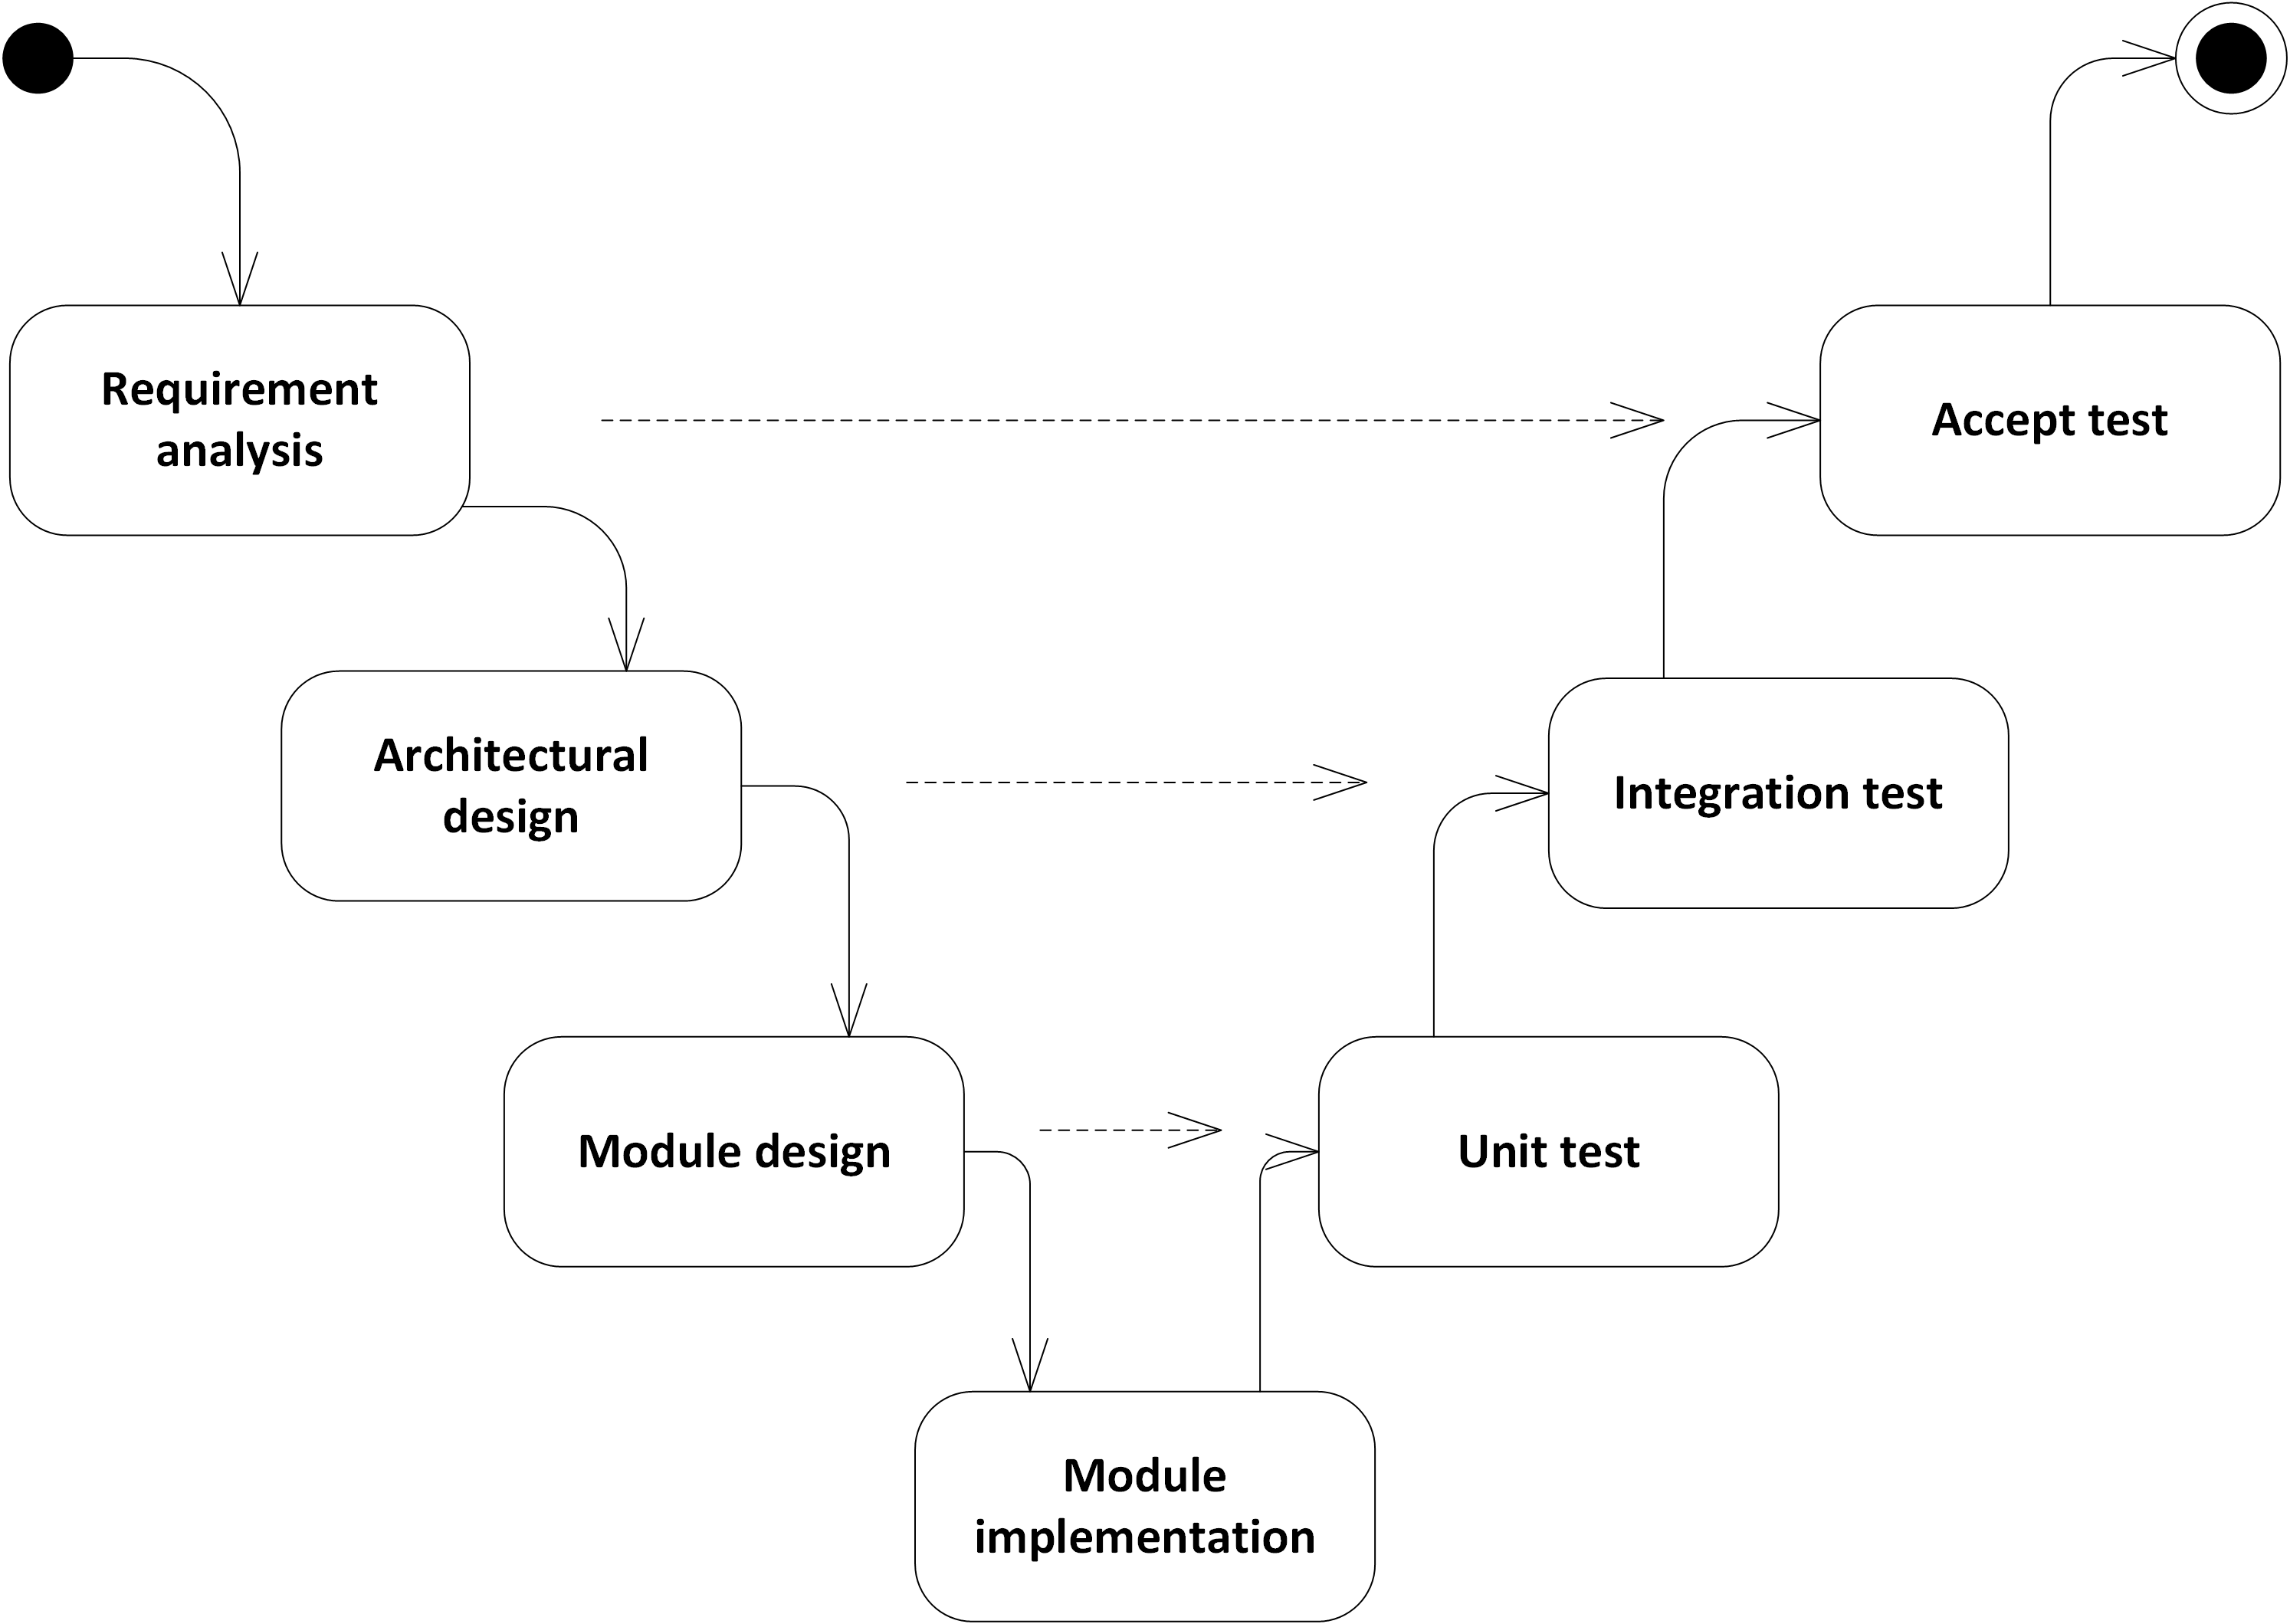
\includegraphics[scale=1.0]{Rapport/VModel.PNG}
	\caption{V-Modellen}
	\label{VModel}
\end{figure} 
Den første udviklingsfase er udarbejdelse af kravspecifikationen. Her udvikles der en tilhørende accepttest, der verificerer systemets overordnede funktionalitet. Den næste fase er systemarkitekturen.
I denne fase udvikles test af integrationen mellem implementerede moduler. Under design og implementering som udgør den sidste fase i udviklingen, udføres der løbende unit test af de implementerede moduler.

\subsection{SCRUM}
Udviklingsmetoden har være Scrum-inspireret, men da processen ikke har været fuld ud tilrettelagt, er det ikke ren Scrum. En af grundene har været at processen bliver uforudsigelig, når der bruges nye værktøjer og derfor har der været behov for fleksible tidsplaner og hyppig gennemgange. 
\newline
\newline
I dette projekt er metoden blevet anvendt til at dele større opgaver op i små dele til de forskellige sprints, samt til at holde daglige møder om arbejdet og opgaverne. 


\subsection{Change Management}
Der blev brugt en Change Management metode for at sikre, at der ikke kom utilsigtigede ændringer ind. Processen er groft tegnet i \ref{fig:ChangeManagement_SEQ}. Flowet kan bedst beskrives som følger:
\begin{enumerate}[label=\arabic{enumi}.,ref=\arabic{enumi}]
  \item \label{editorstart} En Editor (person der ønsker at lave en ændring) laver nogle ændringer og laver et Pull Request
  \item Github (Se \ref{developmentstool}) tager fat i TeamCity serveren(Se \ref{developmentstool}), og informerer at der er kommet et nyt Pull Request
  \item TeamCity serveren bygger og kører unit, integration og fxcop tests. Dette meldes tilbage til Github, samt kan man fra Github gå direkte til build processen på TeamCity serveren.
  \item Hvis der er fejl lukkes Pull Requesten af Reviewer (person der godkender ændringer) og Editor begynder fra \ref{editorstart}.
  \item Hvis alle tests går godt kigger Reviewer ændringerne igennem for at gribe fejl der ikke umiddelbart kan testes for. Dette kunne være unødvendige filer, volapyk der er glemt at blive rettet, ændringer der designmæssigt er forkerte mm.
  \item Hvis ovenstående bliver godkendt af Reviewer, merger Reviewer Pull Requesten og denne lukkes.
  \item Hvis ændringer ikke kan godkendes begynder Reviewer fra \ref{editorstart}.
\end{enumerate}

Et sekundært afkast er at dette hjælper med at mindske, at merge konflikter kommer ind i masteren. Et eksempel kunne være følgende stykke kode.
\begin{lstlisting}
// Vis vores Item paa skaermen
public void ShowItem(Item item, string prefix)
{
    Console.Write(item);
}
\end{lstlisting}
Det kan tydeligt ses at variablen prefix ikke bliver brugt. Person A og B begynder nu begge at ændre på denne fil. Person A fjerner prefix variablen da denne jo ikke er i brug.
\begin{lstlisting}
// Vis vores Item paa skaermen
public void ShowItem(Item item)
{
    Console.Write(item);
}
\end{lstlisting}
Person B derimod har opdaget at han har glemt at bruge prefix, og retter sin fejl.
\begin{lstlisting}
// Vis vores Item paa skaermen
public void ShowItem(Item item, string prefix)
{
    Console.Write(prefix + " " + item);
}
\end{lstlisting}
Begge disse ændringer ville let kunne merges rent teknisk, da ændringerne er langt nok fra hinanden.
\begin{lstlisting}
// Vis vores Item paa skaermen
public void ShowItem(Item item)
{
    Console.Write(prefix + " " + item);
}
\end{lstlisting}
Dog kan filen nu ikke kompileres længere! Dette løses med ovenstående Change Management, da nummer 2 Pull Request ville blive afvist af TeamCity. 
\sysml{0.9}{SEQ}{ChangeManagement}{Change Management}